\documentclass[a4paper,11pt,UTF8]{article}
\usepackage{ctex}
\usepackage{amsmath,amsthm,amssymb,amsfonts}
\usepackage{amsmath}
\usepackage[a4paper]{geometry}
\usepackage{graphicx}
\usepackage{microtype}
\usepackage{siunitx}
\usepackage{booktabs}
\usepackage[colorlinks=false, pdfborder={0 0 0}]{hyperref}
\usepackage{cleveref}
\usepackage{esint} 
\usepackage{graphicx}
\usepackage{ragged2e}
\usepackage{pifont}
\usepackage{extarrows}
\usepackage{mathptmx}
\usepackage{float}
\usepackage{caption}
\usepackage{multirow}
\usepackage{subfigure}
\usepackage{titlesec}
\usepackage{makecell}
\usepackage{tabularx}
\usepackage{graphicx}

\numberwithin{equation}{subsection}
\begin{document}
\tableofcontents\newpage
\section{实验名称}
信号产生与变换电路
\section{实验目的}
\begin{itemize}
	\item 集成运放性能指标含义
	\item 集成运放使用方法与注意事项(调零及频率补偿)
	\item 函数发生器设计方法与测试技术
	\item 两级电路的级联与调试方法	
\end{itemize}
\section{实验元器件}

\begin{table}[h]
	\centering
	\begin{tabular}{|c|c|c|}
		\hline
		名称 & 型号/参数 & 数量\\
		\hline
		运算放大器 & NE5532 & 1\\
		\hline
		\multirow{2}{*}{电容} & 0.1$\mu$F & 1 \\
		\cline{2-3}
		& 0.01$\mu$F & 1\\
		\hline
		\multirow{5}{*}{电阻} & 100kΩ & 2 \\
		\cline{2-3}
		& 47kΩ & 1\\
		\cline{2-3}
		& 20kΩ & 1\\
		\cline{2-3}
		& 10kΩ & 3\\
		\cline{2-3}
		& 5.1kΩ & 1\\
		\hline 		
	\end{tabular}
\end{table}
\section{实验原理}
下图所示的电路能自动产生方波-三角波,图中虚线右边是积分器($A_2$), 虚线左边是同相输入的迟滞电压比较器($A_1$),其中 $C_1$ 称为加速电容,可加速比较器的翻转。电路的工作原理分析如下:
\begin{figure}[H]
	\centering
	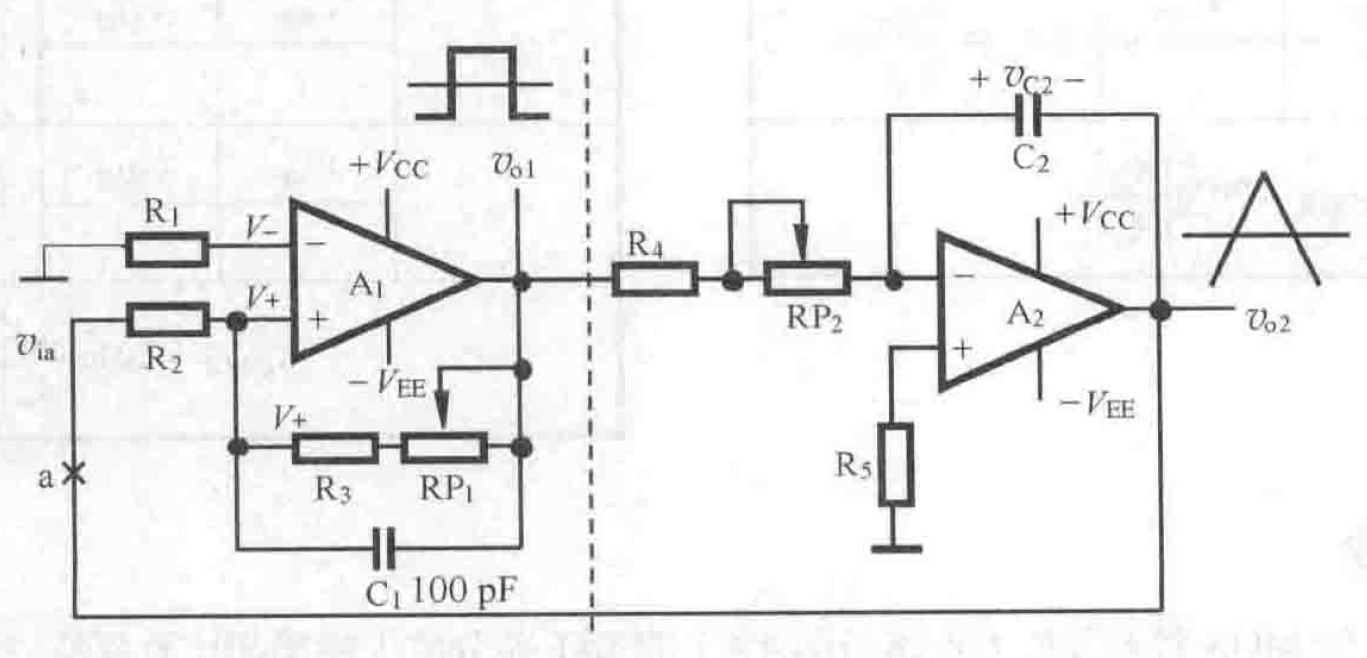
\includegraphics[width=0.7\textwidth]{4}
	\caption{原理图}
\end{figure}
若 a 点断并,比较器 $A_1$的反相端接基准电压,即 $V_-=0$, 同相端接输入电压 $v_\mathrm{ia}$; 比较器输出 $v_\mathrm{ol}$ 的高电平 $v_\mathrm{OH}$ 接近于正电源电压+$\nu_\mathrm{cc}$,低电平 $v_\mathrm{OL}$ 接近于负电源电压-$V_\mathrm{EE}$ (通常$|+V_{CC}|=|-V_{EE}|)$。根据叠加原理,得到:
\begin{align}
	V_{+}=\frac{R_{2}}{R_{2}+R_{3}+\mathrm{RP}_{1}}V_{\mathrm{o1}}+\frac{R_{3}+\mathrm{RP}_{1}}{R_{2}+R_{3}+\mathrm{RP}_{1}}V_{\mathrm{ia}}
\end{align}

式中,RP,指电位器的调整值(以下同)。
通常将比较器的输出电压 $v_\mathrm{ol}$ 从一个电平跳变到另一个电平时对应的输入电压称为门限电压。将比较器翻转时对应的条件 $V_+=V_-=0$ 代入式 (4.0.1), 得到
\begin{align}
	V_{\mathrm{ia}}=\frac{-R_{2}}{R_{3}+\mathrm{RP}_{1}}V_{\mathrm{ol}}
\end{align}

设 $V_{\mathrm{ol}}=V_{\mathrm{OH}}=+V_{\mathrm{CC}}$,代入式(4.0.2)得到一个较小值,即比较器翻转的下门限电平
\begin{align}
	V_{\mathrm{T~-}}=V_{\mathrm{ia}_{-}}=\frac{-R_{2}}{R_{3}+\mathrm{RP}_{1}}V_{\mathrm{OH}}=\frac{-R_{2}}{R_{3}+\mathrm{RP}_{1}}V_{\mathrm{CC}}
\end{align}

设$V_{\mathrm{ol}}=V_{\mathrm{OL}}=-V_{\mathrm{EE}}=-V_{\mathrm{CC}}$,代入式(4.0.2)得到一个较大值,即比较器翻转的上门限电平
\begin{align}
	V_{\mathrm{T}+}=V_{\mathrm{ia}+}=\frac{-R_{2}}{R_{3}+\mathrm{RP}_{1}}V_{\mathrm{OL}}=\frac{R_{2}}{R_{3}+\mathrm{RP}_{1}}V_{\mathrm{CC}}
\end{align}

比较器的门限宽度或回差电压为
\begin{align}
	\Delta V_{\mathrm{T}}=V_{\mathrm{T+}}-V_{\mathrm{T-}}=2\times\frac{R_{2}}{R_{3}+\mathrm{RP}_{1}}V_{\mathrm{CC}}
\end{align}

比较器的电压传输特性如图2(a)所示。当$v_\mathrm{ia}$为往复跨越上、下门限电平的电压波形时,则 $v_\mathrm{ol}$ 不断在高、低电平之间跳变,即输出一串方波。$C_1$在 $v_\mathrm{ol}$ 跳变瞬间可看作短路,使门限迅速改变,即运放 $A_1$的 $\nu_+$和 $\nu$之差迅速增大,从而加速输出的翻转。$C_1$在 $\upsilon_\mathrm{ol}$ 保持高电平或低电平期间则可看作开路。
\begin{figure}[H]
	\centering
	\subfigure[比较器电压传输特性]{
		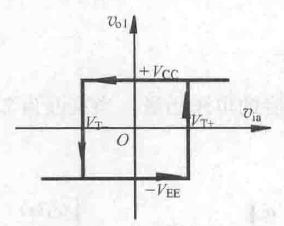
\includegraphics[width=0.3\textwidth]{4.1}
	}
	\subfigure[方波-三角波]{
		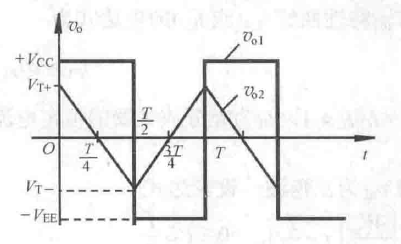
\includegraphics[width=0.4\textwidth]{4.2}
	}
	\caption{}
\end{figure}
a 点断开后,运放 $A_2$与 $R_4$、$RP_2$、$C_2$及 $R_5$组成反相积分器,若积分器的输入信号 $v_\mathrm{ol}$ 为方波,则输出电压等于电容两端的电压,即
\begin{align}
	v_{02}& =-v_{\mathrm{C2}}=-\frac{1}{C_{2}}\int\frac{v_{\mathrm{ol}}}{(R_{4}+\mathrm{RP}_{2})}\mathrm{d}t=-\frac{1}{C_{2}}\int_{t_{0}}^{t_{1}}\frac{v_{\mathrm{ol}}}{(R_{4}+\mathrm{RP}_{2})}\mathrm{d}t-v_{\mathrm{C2}}(t_{0})\nonumber\\ &=-\frac{v_{\mathrm{ol}}}{(R_{4}+\mathrm{RP}_{2})C_{2}}(t_{1}-t_{0})+v_{02}(t_{0})
\end{align}

式中,$v_{\mathrm{C2}}(t_0)$是$t_0$时刻电容两端的初始电压值,$v_{\mathrm{o2}}(t_0)$是 $t_0$ 时刻电路的输出电压,且有 $v_{\mathrm{o2}}(t_0)=$ $-v_{C2}(t_0)$。

当$v_{01}=+V_{CC}$时,则
\begin{align}
	v_{o2}=-\frac{V_{\mathrm{CC}}}{(R_{4}+\mathrm{RP}_{2})C_{2}}\big(t_{1}-t_{0}\big)+v_{02}\big(t_{0}\big)
\end{align}

当$v_{01}=+V_{CC}$时,则
\begin{align}
	v_{02}=\frac{V_{\mathrm{CC}}}{(R_{4}+\mathrm{RP}_{2})C_{2}}\big(t_{1}-t_{0}\big)+v_{02}\big(t_{0}\big)
\end{align}

可见,当积分器的输入为方波时,输出是一个下降速率与上升速率相等的三角波,其波形关系如图2(b)所示。

a 点闭合,即比较器与积分器首尾相连,形成闭环电路,只要积分器的输出电压 $\upsilon_\mathrm{o2}$ 达到比较器的门限电平,使得比较器的输出状态发生改变,则该电路就能自动产生方波-三角波。

由图 4.5.4 所示的波形可知,输出三角波的峰-峰值就是比较器的门限宽度,即
\begin{align}
	V_{\mathrm{o2pp}}=\Delta V_{\mathrm{T}}=\frac{2R_{2}}{R_{3}+\mathrm{RP}_{1}}V_{\mathrm{CC}}
\end{align}

积分电路的输出电压 $v_\mathrm{oz}$从 $\nu_\mathrm{T}-$上升到 $\nu_\mathrm{T+}$所需的时间是振荡周期的一半,即在 T/2 时间内 $v_\mathrm{o2}$ 的变化量等于$V_\mathrm{o2pp}$。根据式(4.5.8)得到电路的振荡周期为
\begin{align}
	T=\frac{4R_2(R_4+\mathrm{RP}_2)C_2}{R_3+\mathrm{RP}_1}
\end{align}

方波-三角波的频率为
\begin{align}
	f=\frac{1}{4(R_4+\mathrm{RP}_2)C_2}\cdot\frac{R_3+\mathrm{RP}_1}{R_2}
\end{align}

由式(4.0.9)及式(4.0.11)可以得出以下结论: 

\ding{172} 方波的输出幅度约等于电源电压+$\nu_\mathrm{cC}$, 三角波的输出幅度与电阻$R_2$与($R_3+{RP}_1)$ 的比值有关,且小于电源电压+$\nu_\mathrm{\epsilon C}$。电位器 RP$_{1}$可实现三角波幅度微调,但会影响方波-三角波的频率。

\ding{173} 电位器 RP$_{2}$ 在调整输出信号的频率时,不会影响三角波输出电压的幅度。因此应先调整电位器 RP$_1$, 使输出三角波的电压幅值达到所要求的值,然后再调整电位器 RP$_2$, 使输出频率满足要求。若要求输出频率范围较宽,可取不同的$C_{2}$来改变频率的范围,用 RP$_{2}$实现频率微调。


\section{实验任务:方波-三角波函数发生器设计}
\noindent 已知条件:运放NE5532一只。

\noindent 性能指标要求:
\begin{itemize}
	\item 频率范围:100 Hz$\sim$1kHz,1kHz$\sim$10 kHz;
	\item 输出电压:方波$V_{pp}$≤24V,三角波$V_{pp}$=6V;
	\item 波形特性:方波$t_r<30\mathrm{\mu s}$(1kHz,最大输出时)三角波$\gamma_\Delta<2\%$
\end{itemize}
注意事项:
\begin{enumerate}
	\item 组装电路前须对所有电阻逐一测量,作好记录。 
	\item 集成运算放大器的各个管脚不要接错,尤其是正、负电源不能接反,否则极易损坏芯片。。
\end{enumerate}
装调步骤:
\begin{enumerate}
	\item 由于比较器$A_1$与积分器$A_2$组成正反馈闭环电路,同时输出方波与三角波,故这两个单元电路需同时安装。
	\item 注意: 在安装电位器RP$_1$与RP$_2$之前,先将其调整到设计值,否则电路可能会不起振。
	\item 如果电路接线正确,则在接通电源后,$A_1$的输出$v_{o1}$为方波,$A_2$的输出$v_{o2}$为三角波。
	\item 在频率较低时,微调RP$_1$,使三角波输出幅度满足设计指标要求。
	\item 再调节RP$_2$,则输出频率连续可变。
	
\end{enumerate}


\section{实验结果}
\subsection{实验记录表格}
\begin{table}[H]
	\centering
	\begin{tabular}{|c|c|c|c|c|}
		\hline
		电容值&方波频率&方波峰峰值/V&	三角波峰峰值/V	&方波上升时间/us\\
		\hline
		\multirow{2}{*}{$C_2=0.1\mu$F} & 994.6Hz & 21.40 & 5.920 & $10.10\mu$s?\\
		\cline{2-5}
		& 100.4Hz & 21.80 & 6.00 & $26.10\mu$s?\\
		\hline
		\multirow{2}{*}{$C_2=0.01\mu$F} & 1.034kHz & 21.80 &  6.000 & $8.086\mu$s?\\
		\cline{2-5}
		& 10.27kHz & 21.00 &  6.480 & $7.609\mu$s?\\
		\hline
	\end{tabular}
\end{table}
\subsection{实验图像(对应表格)}
100 Hz$\sim$1kHz

\begin{figure}[H]
	\centering
	\subfigure{
		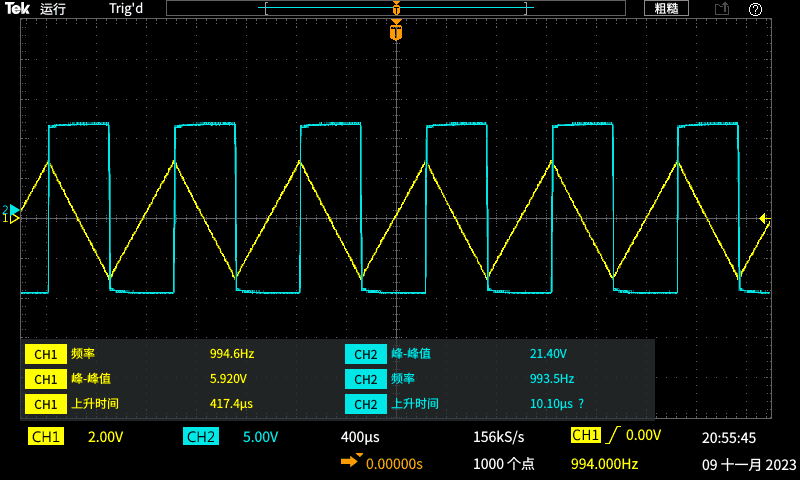
\includegraphics[width=0.48\textwidth]{TEK00018}
	}
	\subfigure{
		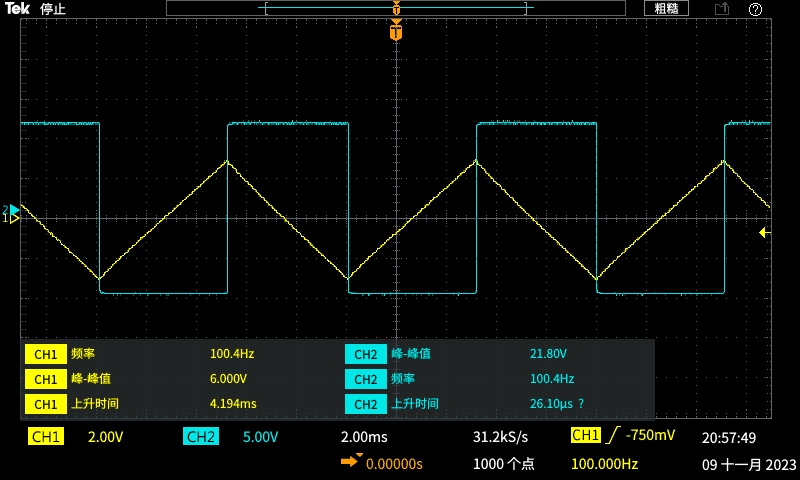
\includegraphics[width=0.48\textwidth]{TEK00019}
	}
\end{figure}
1kHz$\sim$10 kHz
\begin{figure}[H]
	\centering
	\subfigure{
		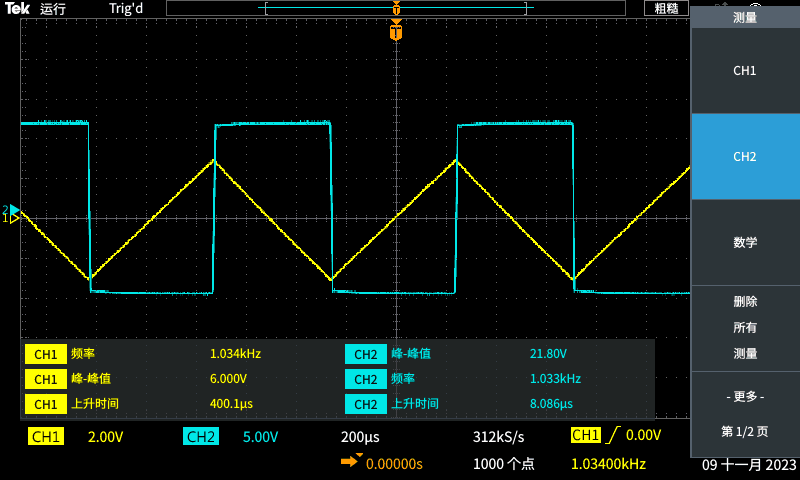
\includegraphics[width=0.48\textwidth]{TEK00015.PNG}
	}
	\subfigure{
		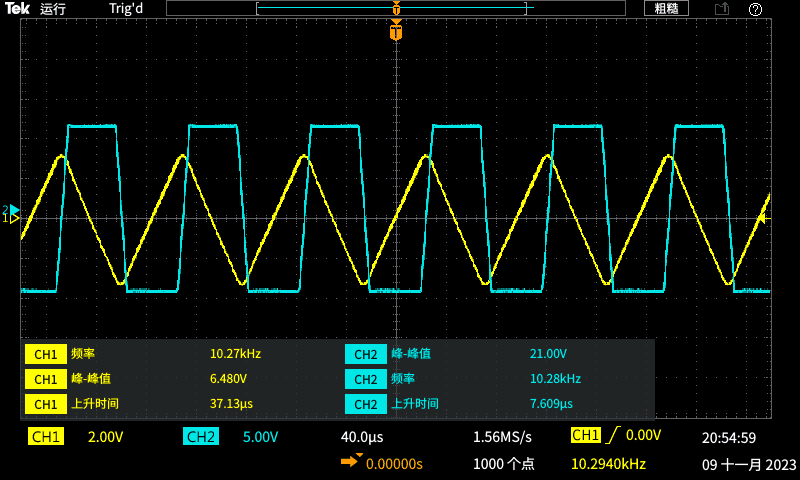
\includegraphics[width=0.48\textwidth]{TEK00017.PNG}
	}
\end{figure}
\subsection{实验结果}
方波的幅度由+$V_{CC}$和–$V_{EE}$决定,小于它们1V左右;三角波幅度可由RP1进行调节,但会影响频率。调节RP2,可调节频率,且不会影响三角波幅度,可用RP2实现频率微调,用C2改变频率范围。

误差分析:

实验误差很大程度来自于电容,实验器材中提供的104陶瓷电容误差过大,导致调整挡位无法调到合理频率范围,最后通过两个104电容并联基本完成了实验要求。
\section{实验小结}
本次实验电路搭建遇到了一点问题,当按照要求搭完电路后,并不能产生要求的波形,反复检查多次电路没有发现问题,最后无奈通过重新搭建电路解决了问题。

同时,在重新搭建电路的过程中,我采用了分左右两块进行搭建的方法,确保能够产生实验需要的波形。
\end{document}